% Completa los datos convenientemente en las zonas marcadas con TODO

\documentclass{beamer}
%PARA VISUALIZAR PRESENTACIONN CON NOTAS USAR VISUALIZADOR "pdfpc":
%Para ver las notas, el cronometro y siguente diapo:
% pdfpc --notes=right slides.pdf
% "tecla p": para pausar el cronometro
\mode<presentation> {
  \usetheme{CambridgeUS}
  \usecolortheme{crane} % color naranja
}
\setbeamercolor{titlelike}{parent=structure,bg=yellow!85!orange} % Cambia el color de la caja del título de la página inicial

\setbeamertemplate{navigation symbols}{} % ocultar iconos de navegación
\setbeamerfont{subsection in toc}{size=\small} % reducir tamaño en TOC
\setbeamerfont{date}{size=\tiny}
\usepackage[spanish]{babel}
\usepackage[utf8]{inputenc}
\usepackage{graphicx}
\usepackage{booktabs}
\usepackage{hyperref}
\usepackage{multicol}
\usepackage{pgfpages}
\usepackage{listings}
\usepackage{multimedia}
\usepackage[export]{adjustbox}
\usepackage{outlines} % Para poner bullets tabulados (\1 \2 \3 ...) y no items

\usepackage{array,tabularx} % para tabular leyenda de ecuaciones
\newenvironment{conditions*} % entorno de "leyenda de ecuación"
  {\par\vspace{\abovedisplayskip}\noindent
   \tabularx{\columnwidth}{>{$}l<{$} @{\ : } >{\raggedright\arraybackslash}X}}
  {\endtabularx\par\vspace{\belowdisplayskip}}
  
% USO DE NOTAS
\setbeameroption{hide notes} % Para mostrar u ocultar (hide/show)
%\setbeameroption{show only notes} % Mostrar solo las notas
%\setbeameroption{show notes on second screen=right} % Mostrar notas en otra pantalla
\setbeamertemplate{note page}{ % asi solo muestro el texto de las notas
  \insertnote%
}

%========= TODO: datos internos del documento
\hypersetup{
	pdftitle={Defensa de trabajo de fin de grado de Pon tu nombre},
	pdfauthor={Pon tu nombre},
	pdfsubject={Pon aquí el título completo del trabajo},
	pdfkeywords={teaching, robotics, vision, sensors, actuators, raspberry},
	pdfproducer={pdfLaTeX},
  colorlinks=true,
  linkcolor=blue
}
%=========

%========= TODO: diapositiva de portada
\title[Robot de bajo coste guiado por voz]{Prototipo de robot de bajo coste guiado por voz con técnicas de localización} % El título reducido aparece en la parte inferior de todas las diapositivas
                                         % El título completo aparece solo en la diapositiva de portada
\author[Víctor de la Torre Rosa]{Víctor de la Torre Rosa}
\institute[URJC]
{
\textit{\href{mailto:escribe.tu@correo.es}{\color{blue}{\underline{v.delatorre.2019@alumnos.urjc.es}}}}\\
\vspace{0.5cm}

\includegraphics[width=3cm]{figs/logo-urjc}\\
\vspace{1cm}
Trabajo Fin de Grado
}
\date{xx de xxxxxxx de 20xx}
%=========

%========= COMIENZO DEL DOCUMENTO
\begin{document}

%========= Portada inicial con notas
\begin{frame}[plain] % plain: quita header y footer
\large{\titlepage}
\note[item]{En esta presentación voy a hablar sobre...}
\note[item]{En primer lugar...}
\end{frame}

%========= Licencia
\begin{frame}
% Este diseño se corresponde con la licencia CC-BY-NC-SA.
% Por supuesto, puedes poner la licencia que mejor se adapte al propósito de tu trabajo.
% Recuerda que, si no se especifica ninguna licencia, esta -como cualquier creación artística- pasaría a estar licenciada con todos los derechos reservados (copyright).

\cleardoublepage

\begin{flushright}
\begin{figure}
 \ \ \ \ 
\includegraphics[width=0.25\linewidth,right]{figs/by-sa.png}
 \label{fig:cc} 
 \end{figure}
\end{flushright}

\

\

\

\noindent
Este trabajo se distribuye bajo los términos de la licencia internacional \href{http://creativecommons.org/licenses/by-sa/4.0/}{CC BY-SA International License} (Creative Commons Attribution-ShareAlike 4.0). Usted es libre de \textit{(a) compartir}: copiar y redistribuir el material en cualquier medio o formato para cualquier propósito, incluso comercialmente; y \textit{(b) adaptar}: remezclar, transformar y construir a partir del material para cualquier propósito, incluso comercialmente. La licenciante no puede revocar estas libertades en tanto usted siga los términos de la licencia:

\begin{itemize}
\item \textit{Atribución}. Usted debe dar \href{https://creativecommons.org/licenses/by-sa/4.0/deed.es#ref-appropriate-credit}{crédito de manera adecuada}, brindar un enlace a la licencia, e indicar \href{https://creativecommons.org/licenses/by-sa/4.0/deed.es#ref-indicate-changes}{si se han realizado cambios}. Puede hacerlo en cualquier forma razonable, pero no de forma tal que sugiera que usted o su uso tienen el apoyo de la licenciante.
\item \textit{Compartir igual}. Si remezcla, transforma o crea a partir del material, debe distribuir su contribución bajo la \href{https://creativecommons.org/licenses/by-sa/4.0/deed.es#ref-same-license}{misma licencia} del original.\\
No hay restricciones adicionales — No puede aplicar términos legales ni \href{https://creativecommons.org/licenses/by-sa/4.0/deed.es#ref-technological-measures}{medidas tecnológicas} que restrinjan legalmente a otras a hacer cualquier uso permitido por la licencia.
\end{itemize}

\begin{flushright}
		\vspace{7.0 cm}
		\emph{Documento de} \textbf{Víctor de la Torre Rosa}. % TODO: pon aquí tu nombre cuando hagas el documento
\end{flushright}


\end{frame}

%========= Índice o tabla de contenidos (TOC)
\begin{frame}
\frametitle{Contenidos}
%\begin{multicols}{2} % si tengo muchas secciones, lo parte en dos columnas
  \tableofcontents[hideallsubsections] % no muestra subsecciones
%\end{multicols}
\note[item]{La presentaci\'on esta dividida en cuatro partes.}
\end{frame}

%========= Diapositiva "vacía" de comienzo de sección:
\section*{}
\begin{frame}{}
  \centering \Huge
  \emph{Introducción}
\note[item]{Comencemos con la introducción.}
\end{frame}

\section{Introducción}
\subsection{Contexto general}
%========= Diapositiva con imágenes:
\begin{frame}
\frametitle{Robótica móvil}
\centering
\begin{minipage}{0.45\textwidth}
    \centering
    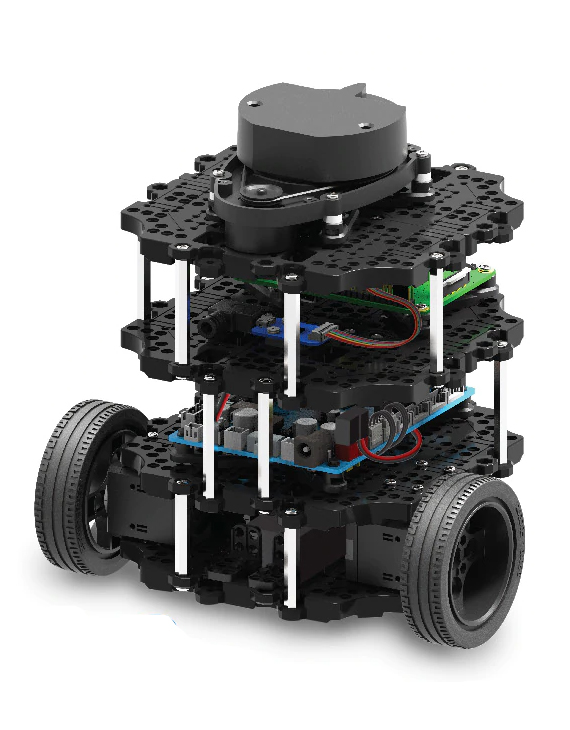
\includegraphics[width=3.4cm]{figs/turtlebot3burguer.jpg}
\end{minipage}
\hfill
\begin{minipage}{0.45\textwidth}
    \centering
    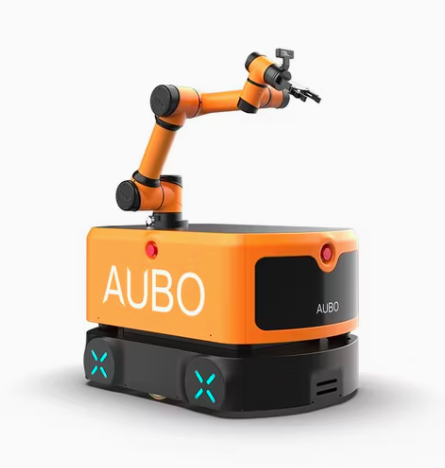
\includegraphics[width=3.4cm]{figs/ttt.png}
\end{minipage}
\end{frame}





%========= Diapositiva con ítems resaltados con colores:
\begin{frame}
\frametitle{Robótica educativa y de bajo coste}
\centering

% Primera fila
\begin{minipage}{0.45\textwidth}
    \centering
    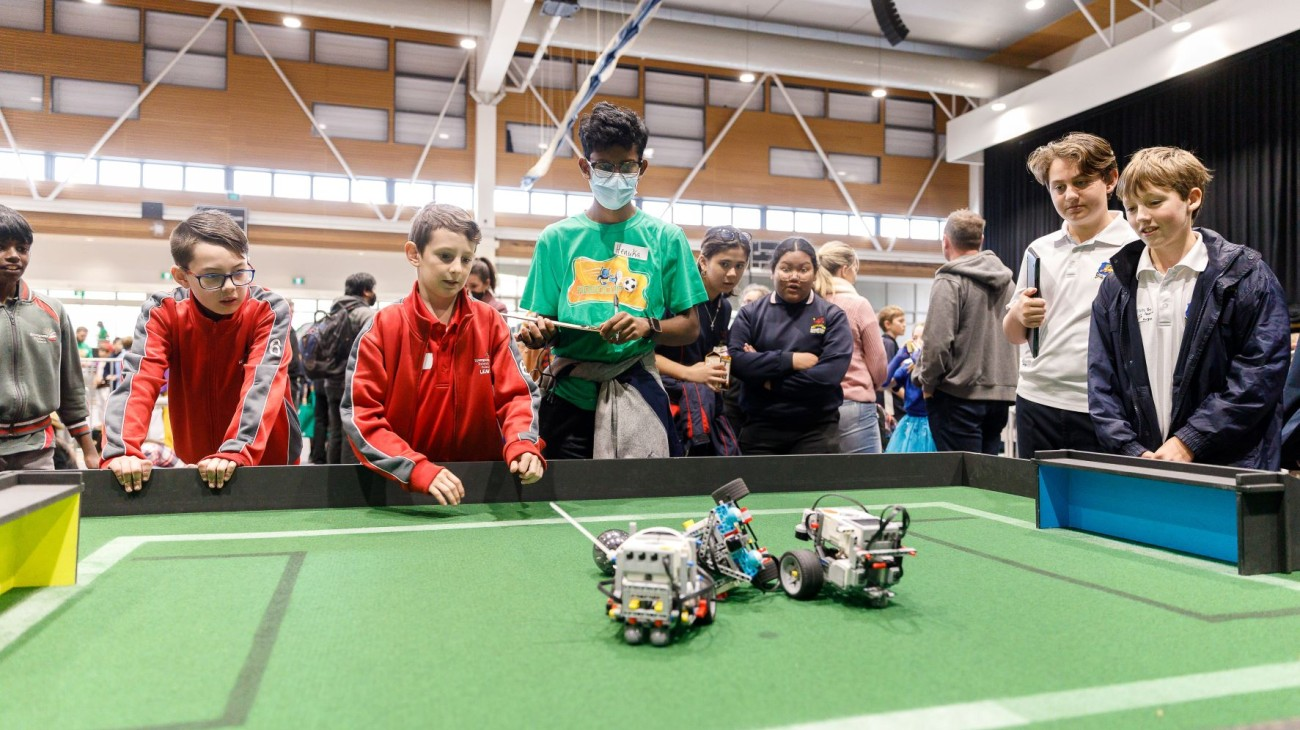
\includegraphics[width=3.4cm]{figs/RoboCup_junior.jpg}
\end{minipage}
\hfill
\begin{minipage}{0.45\textwidth}
    \centering
    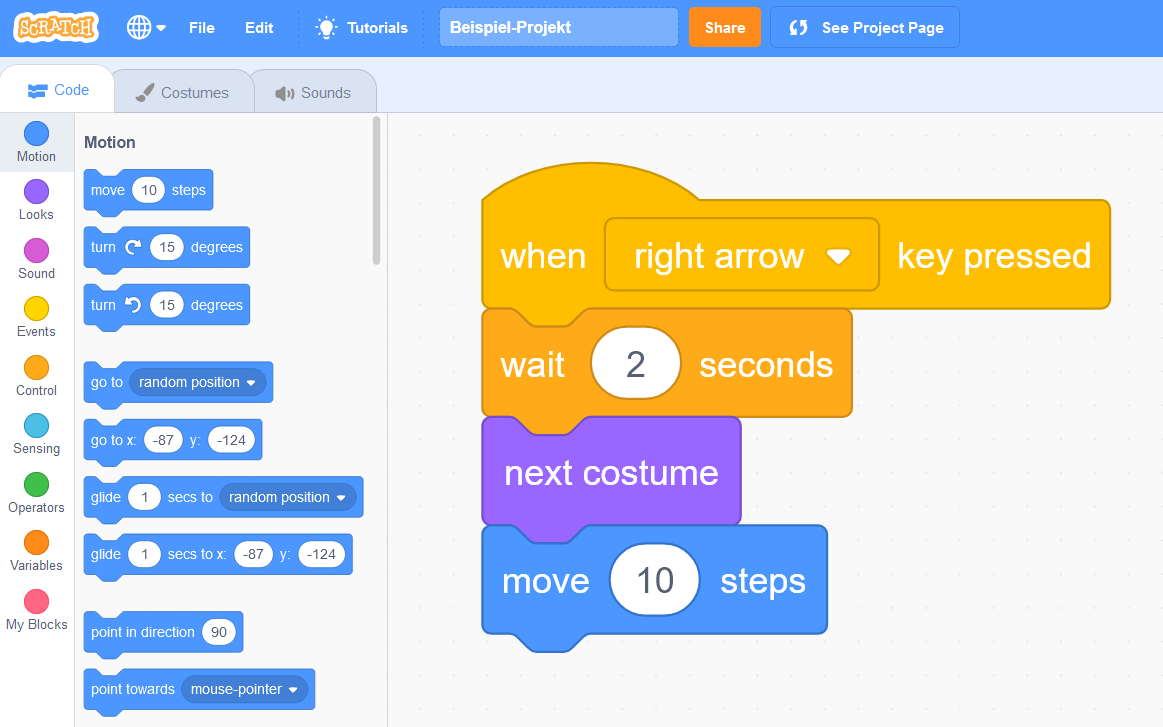
\includegraphics[width=3.4cm]{figs/scratch.png}
\end{minipage}

\vspace{0.5cm} % Espacio entre filas

% Segunda fila
\begin{minipage}{0.45\textwidth}
    \centering
    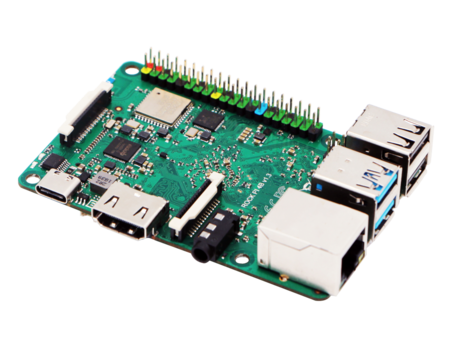
\includegraphics[width=3.4cm]{figs/raspberry4.png} % Cambia por la ruta de la tercera imagen
\end{minipage}
\hfill
\begin{minipage}{0.45\textwidth}
    \centering
    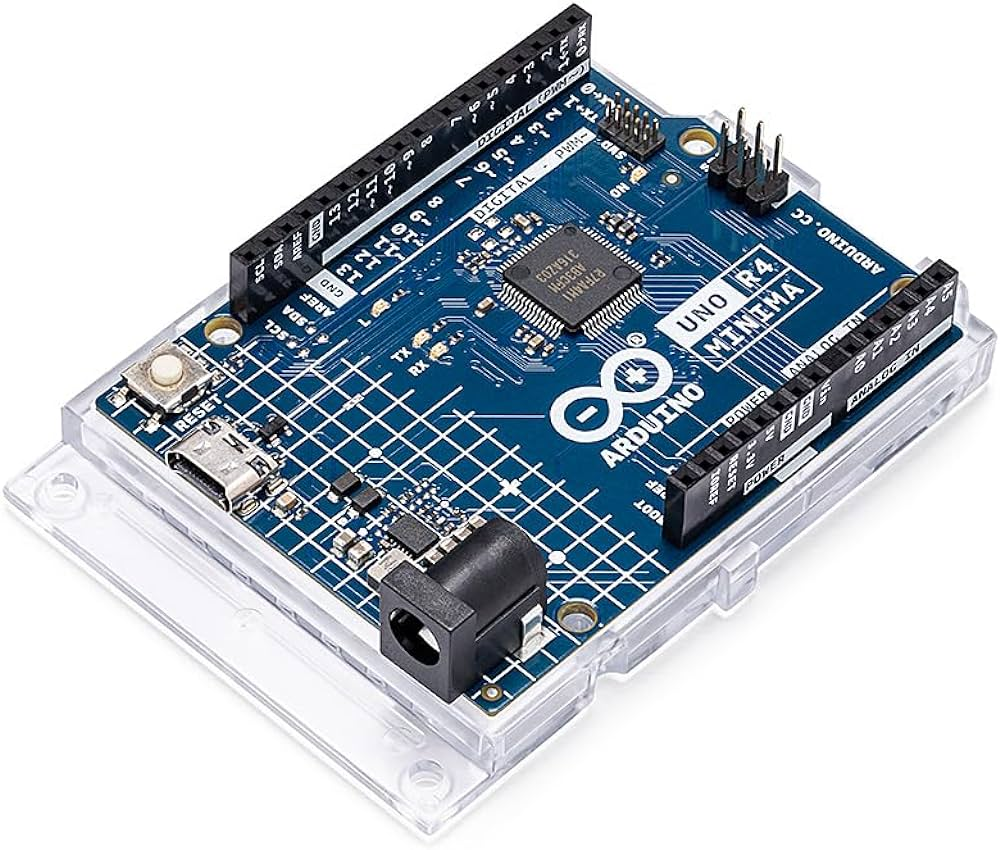
\includegraphics[width=3.4cm]{figs/arduino_uno.jpg} % Cambia por la ruta de la cuarta imagen
\end{minipage}

\end{frame}



\section*{}
\begin{frame}{}
  \centering \Huge
  \emph{Objetivos}
\note[item]{Pasemos ahora a comentar los objetivos que nos hemos con este trabajo.}
\end{frame}

\section{Objetivos}
\begin{frame}
\frametitle{Descripción del problema}
\centering

% Primera fila
\begin{minipage}{0.45\textwidth}
    \centering
    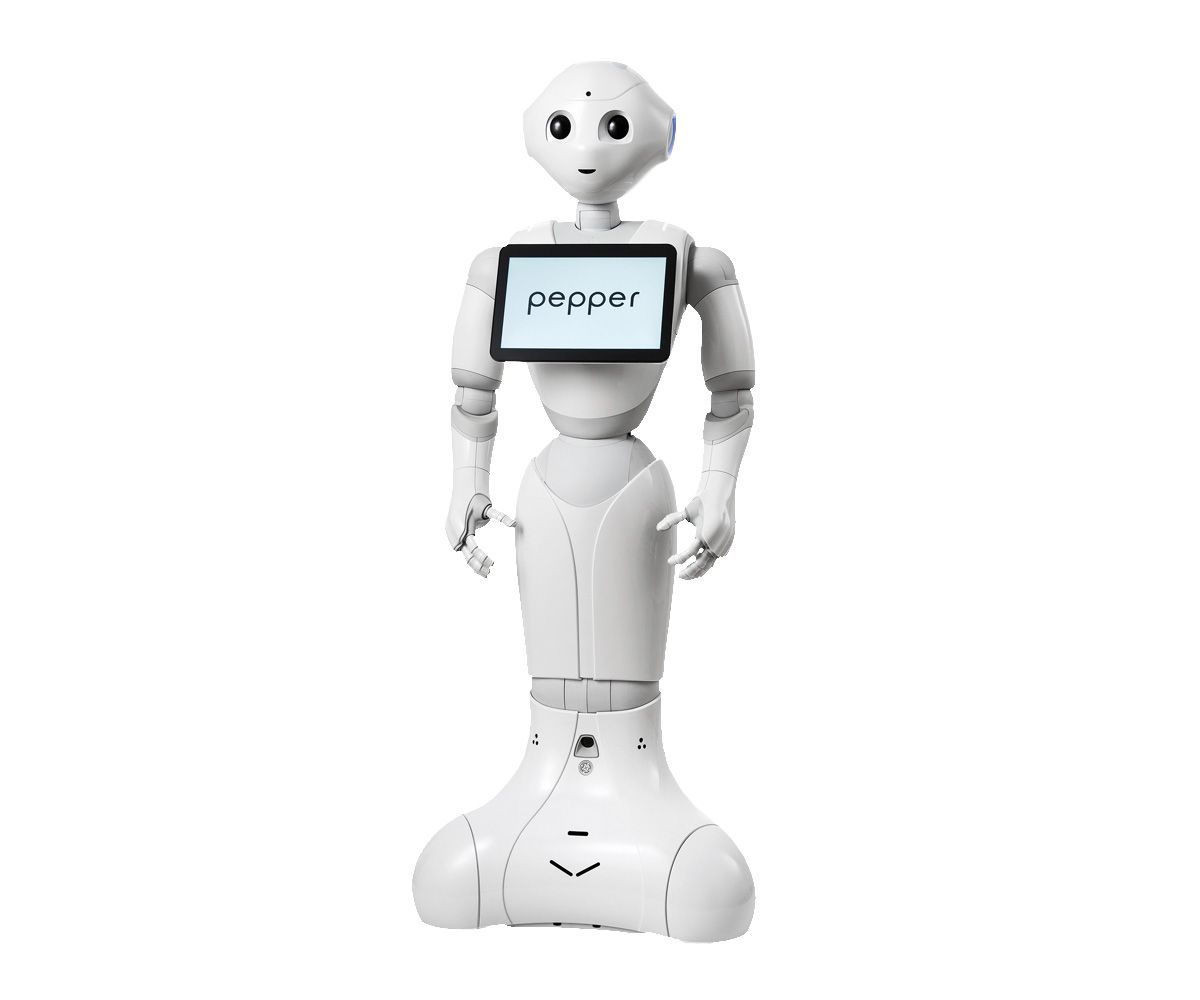
\includegraphics[width=4.4cm]{figs/peper.jpg}
\end{minipage}
\hfill
\begin{minipage}{0.45\textwidth}
    \centering
    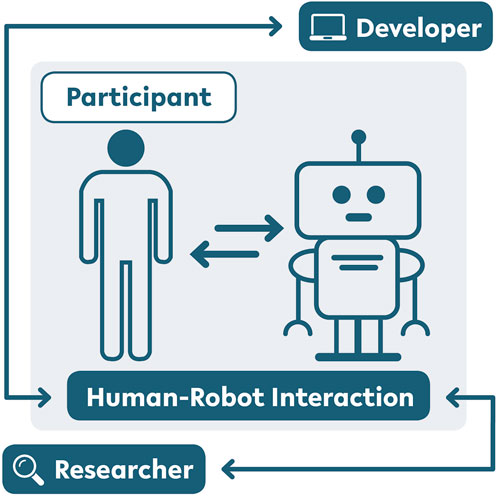
\includegraphics[width=3.8cm]{figs/hri.jpg}
\end{minipage}

\vspace{0.5cm} % Espacio entre filas

% Segunda fila
\begin{minipage}{0.45\textwidth}
    \centering
    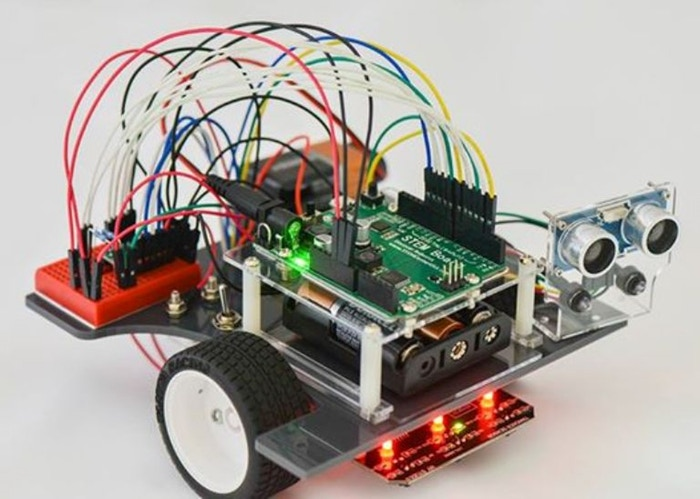
\includegraphics[width=3.8cm]{figs/robot_rasp.jpg} % Cambia por la ruta de la tercera imagen
\end{minipage}
\hfill
\begin{minipage}{0.45\textwidth}
    \centering
    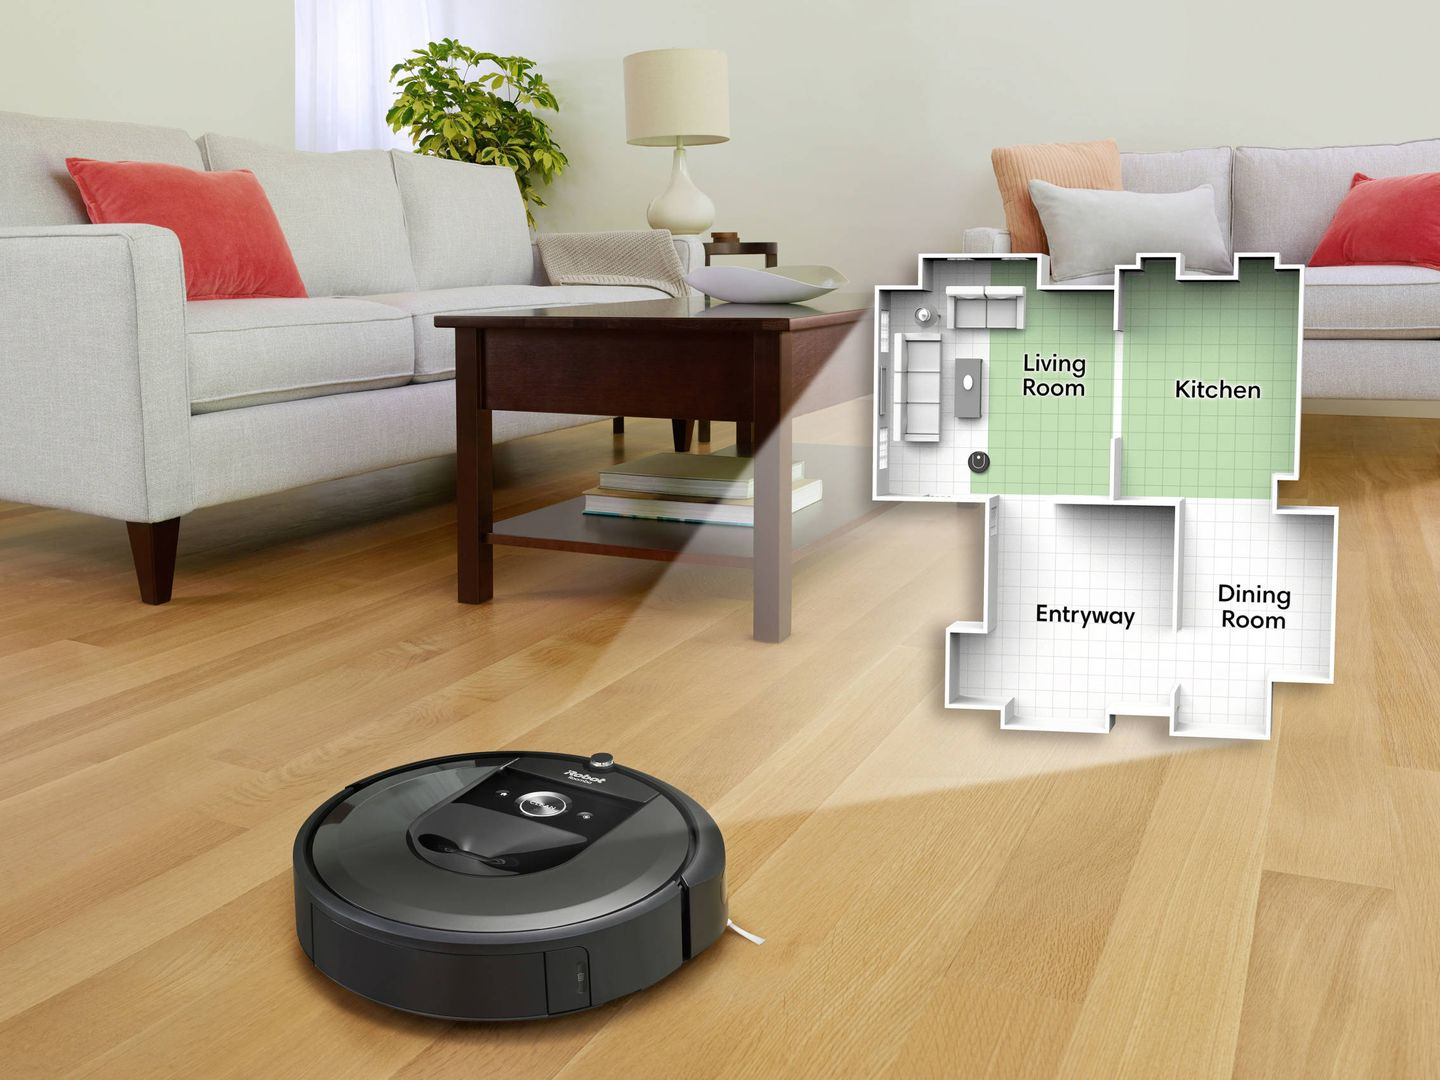
\includegraphics[width=3.8cm]{figs/rumba.jpg} % Cambia por la ruta de la cuarta imagen
\end{minipage}

\end{frame}

\section{Plataforma de desarrollo}
\begin{frame}
\frametitle{Requisitos}
\begin{enumerate}
\item Coste inferior a 145€.
\item Hardware económico.
\item Disponer de varios puntos de acceso Wi-Fi.
\item Uso de una impresora convencional para las piezas.
\item El sistema debe ser capaz de ejecutar en tiempo real sobre Raspberry.
\item El lenguaje de programación debe ser Python.
\item Batería recargable.
\item Los motores y la batería deben de pesar lo menos posible.
\end{enumerate}
\end{frame}

\begin{frame}
\frametitle{Objetivos específicos}
\begin{enumerate}
\item Explorar diferentes opciones de diseño.
\item Realizar una investigación sobre los distintos componentes tanto hardware como software.
\item Gestionar el control del prototipo desde el ordenador.
\item Poder combinar los datos de navegación y localización sin que intervengan
unos con otros mediante la librería threading.
\item Realizar la calibración necesaria de los sensores.
\item Entrenar una red neuronal con audios para enseñar a la red
a clasificar las órdenes.
\end{enumerate}
\end{frame}

\begin{frame}
\frametitle{Metodología}
\centering
\begin{minipage}{0.45\textwidth}
    \centering
    
\includegraphics[width=5.4cm]{figs/git.png}
\end{minipage}
\hfill
\begin{minipage}{0.45\textwidth}
    \centering
    
\includegraphics[width=3.2cm]{figs/teams.png}
\end{minipage}
\end{frame}

\section*{}
\begin{frame}{}
  \centering \Huge
  \emph{Plataforma de desarrollo}
\note[item]{Una vez descritos los objetivos, veamos qué hemos hecho para alcanzarlos.}
\end{frame}

\section{Plataforma de desarrollo}
\section{Plataforma de desarrollo}
\begin{frame}
\frametitle{Hardware}
\centering

% Primera fila
\begin{minipage}{0.3\textwidth}
    \centering
    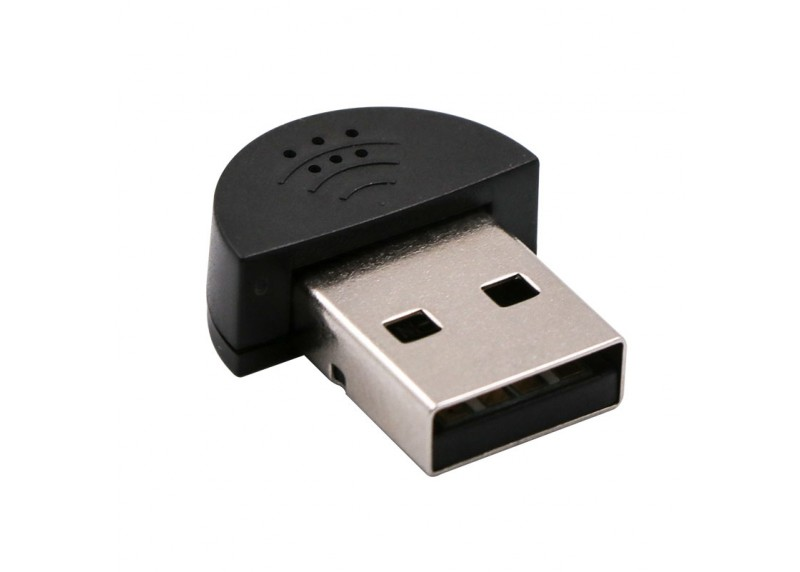
\includegraphics[width=2.3cm]{figs/microfono-usb.jpg}
\end{minipage}
\hfill
\begin{minipage}{0.3\textwidth}
    \centering
    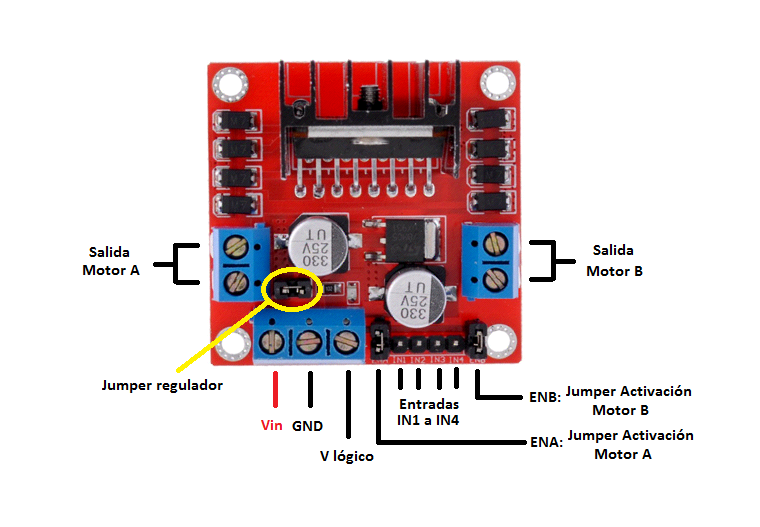
\includegraphics[width=3.0cm]{figs/L298N.png}
\end{minipage}
\hfill
\begin{minipage}{0.3\textwidth}
    \centering
    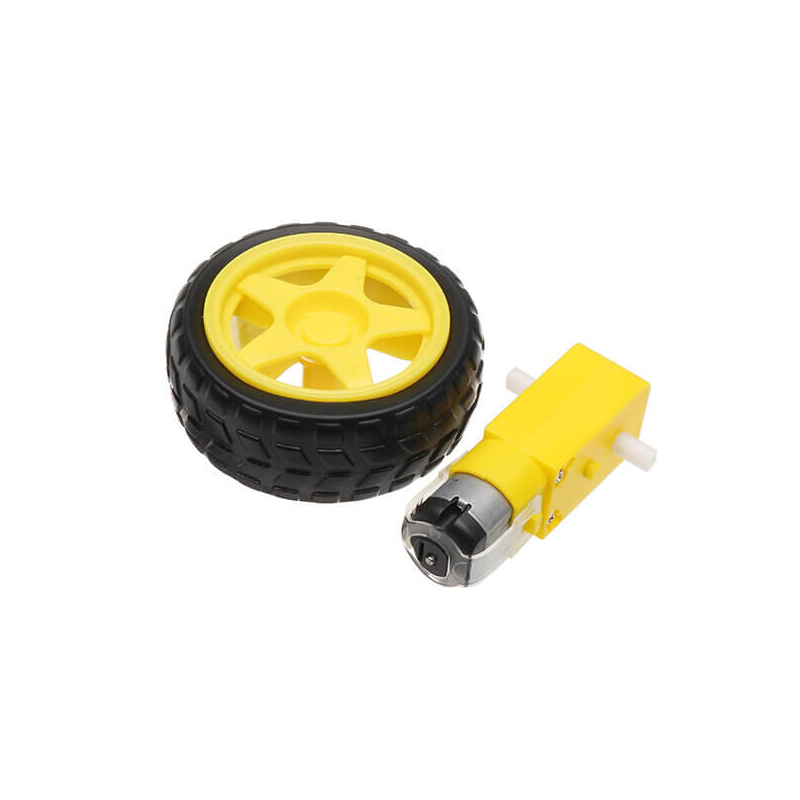
\includegraphics[width=2.6cm]{figs/motor.jpg}
\end{minipage}

\vspace{-0.3cm} % Reduce el espacio entre filas


% Segunda fila
\begin{minipage}{0.3\textwidth}
    \centering
    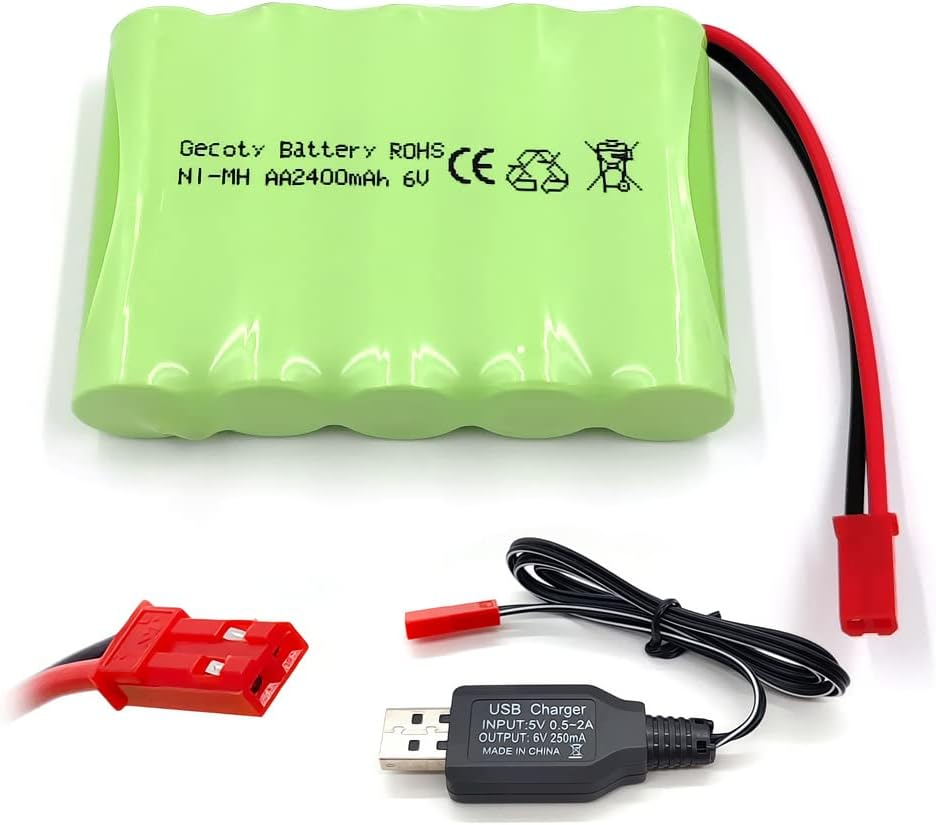
\includegraphics[width=2.0cm]{figs/bateria.jpg} 
\end{minipage}
\hfill
\begin{minipage}{0.3\textwidth}
    \centering
    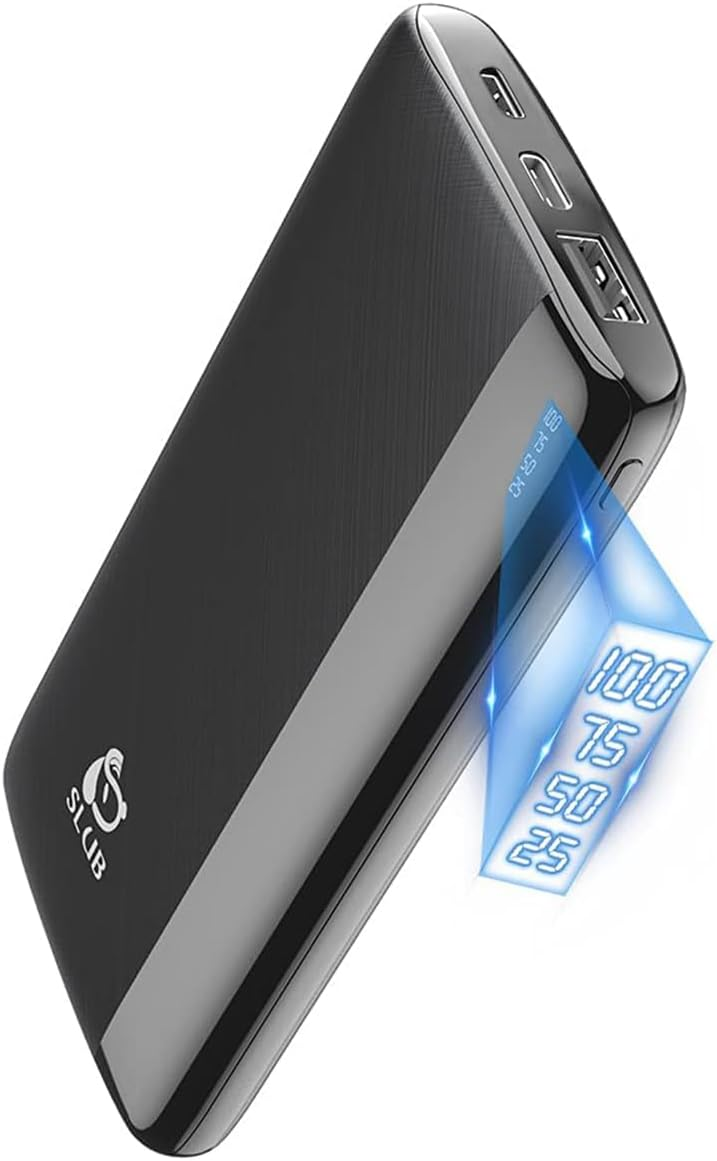
\includegraphics[width=1.1cm]{figs/powerbank.jpg} 
\end{minipage}
\hfill
\begin{minipage}{0.3\textwidth}
    \centering
    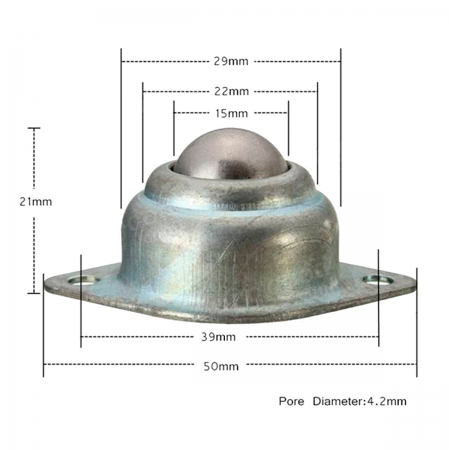
\includegraphics[width=2.0cm]{figs/rueda_loca.png}
\end{minipage}



% Tercera fila
\begin{minipage}{0.3\textwidth}
    \centering
    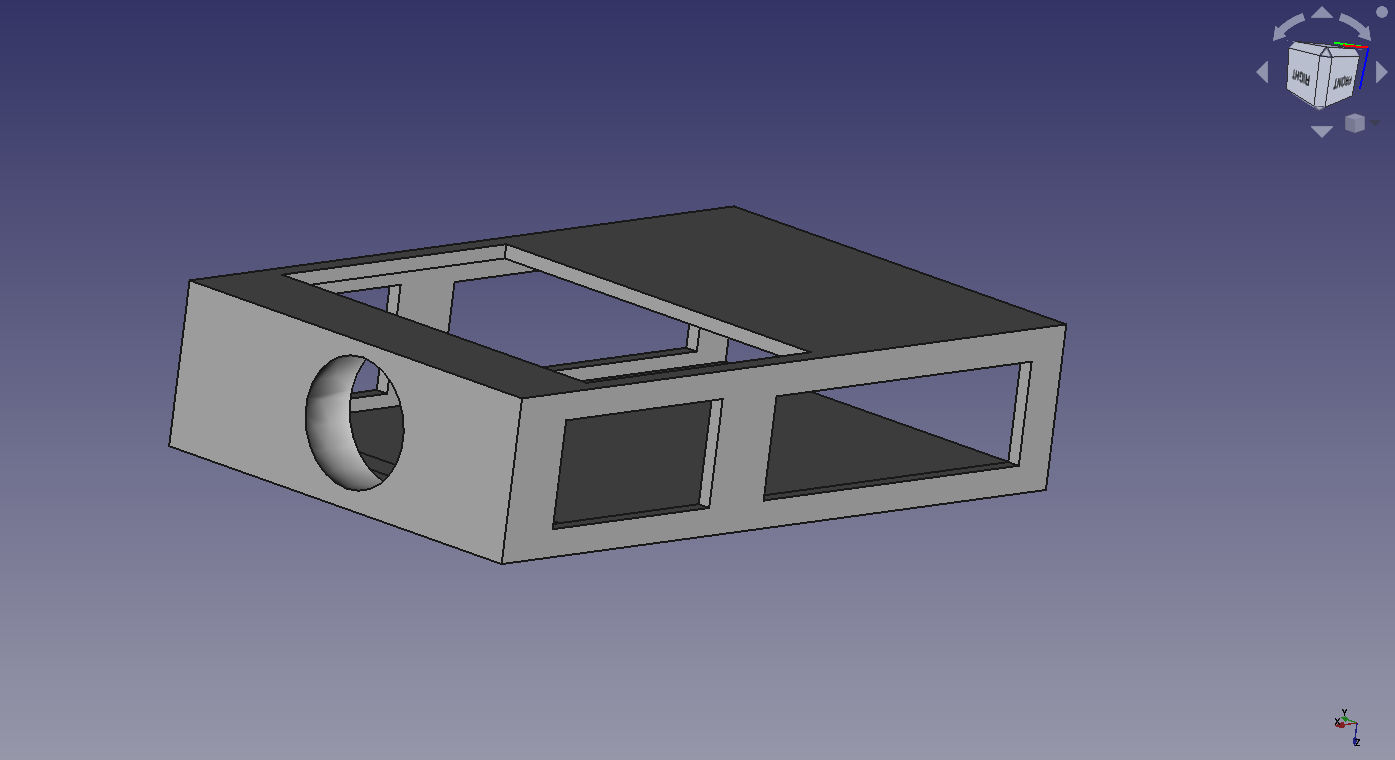
\includegraphics[width=2.3cm]{figs/base.png} 
\end{minipage}
\hfill
\begin{minipage}{0.3\textwidth}
    \centering
    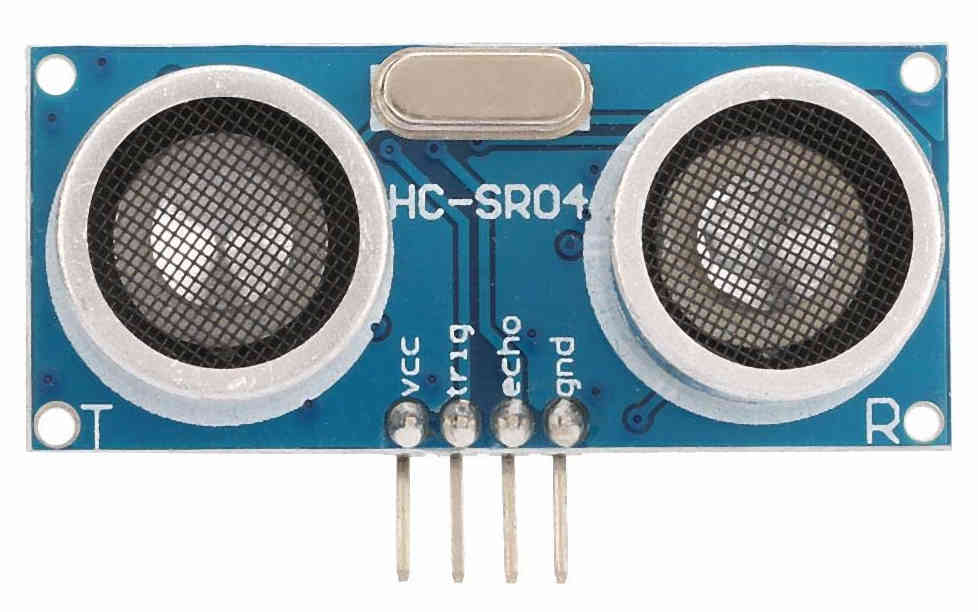
\includegraphics[width=2.0cm]{figs/hcsr04.jpg} 
\end{minipage}
\hfill
\begin{minipage}{0.3\textwidth}
    \centering
    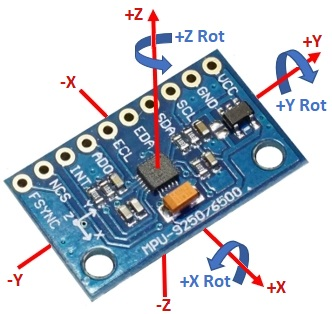
\includegraphics[width=1.8cm]{figs/mpu9250.jpg}
\end{minipage}

\vspace{-0.5cm} % Reduce el espacio entre filas

% Imagen centrada en la última fila
\begin{center}
    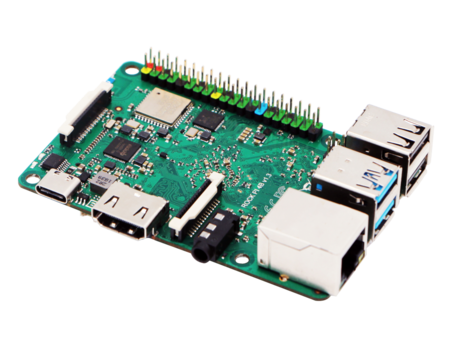
\includegraphics[width=2.7cm]{figs/raspberry4.png}
\end{center}

\end{frame}


%========= Diapositiva con matemáticas y leyenda (conditions*):
\begin{frame}
\frametitle{Software}
\begin{outline}
\1 Si material piezoresistivo se deforma, cambia su resistencia eléctrica.


\1 El cambio de resistencia se obtiene a partir de:

\end{outline}
\end{frame}

%========= Diapositiva con códigos:
\subsection{Algoritmo principal}
\begin{frame}[fragile]
\frametitle{Algoritmo de visión}
\begin{lstlisting}
cvCvtColor (&image, IplTmp1, CV_RGB2GRAY);//to Gray
cvNormalize(IplTmp1, IplTmp1, 0, 255, CV_MINMAX);
cvSmooth(IplTmp1,IplTmp2,CV_BLUR,3,3);//Avrg filter
cvLaplace(IplTmp2, IplLaplace, 3);//Laplace
cvConvertScale(IplLaplace,IplTmp1);
cvThreshold(IplTmp1,IplTmp2,Thress,255,CV_THRESH_BIN);
\end{lstlisting}
\end{frame}

\section*{}
\begin{frame}{}
  \centering \Huge
  \emph{Conclusiones}
\note[item]{Para acabar esta presentación, vamos a repasar lo hecho, unas breves conclusiones y las líneas futuras.}
\end{frame}

\section{Desarrollo software}
\begin{frame}
\begin{block}{Objetivos cumplidos}
\begin{itemize}
\item Herramienta multiplataforma: soporta Linux, Windows, MacOS.
\item Intuitiva para el usuario final: no se necesita instalar nada.
\item Solo se necesita un navegador web.
\end{itemize}
\end{block}

\begin{block}{Líneas futuras}
\begin{itemize}
\item Permitir el uso de otras herramientas.
\item Ampliar los botones disponibles en el interfaz.
\end{itemize}
\end{block}
\end{frame}

\begin{frame}[plain]
\large{\titlepage}
\note[item]{Y hasta aquí mi exposición.}
\note[item]{Quedo a disposición del tribunal...}
\end{frame}

\section{Experimentos}
\begin{frame}
\begin{block}{Objetivos cumplidos}
\begin{itemize}
\item Herramienta multiplataforma: soporta Linux, Windows, MacOS.
\item Intuitiva para el usuario final: no se necesita instalar nada.
\item Solo se necesita un navegador web.
\end{itemize}
\end{block}

\begin{block}{Líneas futuras}
\begin{itemize}
\item Permitir el uso de otras herramientas.
\item Ampliar los botones disponibles en el interfaz.
\end{itemize}
\end{block}
\end{frame}

\begin{frame}[plain]
\large{\titlepage}
\note[item]{Y hasta aquí mi exposición.}
\note[item]{Quedo a disposición del tribunal...}
\end{frame}

\section{Conclusiones}
\begin{frame}
\begin{block}{Objetivos cumplidos}
\begin{itemize}
\item Herramienta multiplataforma: soporta Linux, Windows, MacOS.
\item Intuitiva para el usuario final: no se necesita instalar nada.
\item Solo se necesita un navegador web.
\end{itemize}
\end{block}

\begin{block}{Líneas futuras}
\begin{itemize}
\item Permitir el uso de otras herramientas.
\item Ampliar los botones disponibles en el interfaz.
\end{itemize}
\end{block}
\end{frame}

\begin{frame}[plain]
\large{\titlepage}
\note[item]{Y hasta aquí mi exposición.}
\note[item]{Quedo a disposición del tribunal...}
\end{frame}

\end{document}
